\documentclass{article}[10pt]
\usepackage[utf8]{inputenc}
\usepackage{sectsty}
\allsectionsfont{\bfseries \sffamily}
\usepackage[linkcolor = red]{hyperref}
\usepackage{color}
\usepackage{setspace}
\usepackage{framed}
\usepackage{fancyhdr}
\usepackage{verbatim}
%\documentclass{amsart}
\usepackage{geometry}
\usepackage{alltt}
\usepackage{lastpage}
\usepackage{extramarks}
%\usepackage{mathabx}
\usepackage{parskip}
\usepackage{mathtools}
\usepackage{bbm}
\usepackage{amsfonts}
%\usepackage{titling}
\usepackage{cancel}
\usepackage{chngpage}
\usepackage{tikz}
\usepackage{soul}
\usepackage{array}
\usepackage{sectsty}
\usepackage{ascii}
\usepackage{xcolor}
%\usepackage{mdframed}
\allsectionsfont{\bfseries \sffamily}
%\usepackage{subfig}
%\usepackage{subfigure}
\usepackage{caption}
\usepackage{wrapfig}
\usepackage{subcaption}
\usepackage{enumerate}
\usepackage[usenames,dvipsnames]{color}
\usepackage{graphicx,float,wrapfig}
\usepackage{ifthen}
\usepackage{listings}
\usepackage{setspace}

\geometry{a4paper}

\def\bibindent{2em}

\linespread{2}

\def\changemargin#1#2{\list{}{\rightmargin#2\leftmargin#1}\item[]}
\let\endchangemargin=\endlist

\newcommand{\hmwkTitle}{Final Report}
\newcommand{\hmwkSubTitle}{}
\newcommand{\hmwkDueDate}{}
\newcommand{\hmwkClass}{GEOG 6000}
\newcommand{\hmwkClassTime}{}
\newcommand{\hmwkClassInstructor}{Professor Simon Brewer}
\newcommand{\hmwkAuthorName}{Evan Young}

%\pagestyle{fancy} 

\setlength{\itemindent}{.5in}

% Margins
\topmargin=-0.5in      %
\evensidemargin=-.12in     %
\oddsidemargin=-.12in      %
%\marginparwidth = 0pt
\textwidth=6.5in        %
\textheight=9.25in       %
\headsep=0.25in         %

% Make title
\title{\vspace{2in}\textsf{\textmd{\textbf{{\Huge \hmwkClass:\ \hmwkTitle}\vspace{.2in}\hrule\vspace{.1in}\ifthenelse{\equal{\hmwkSubTitle}{}}{}{\\\hmwkSubTitle}}}\\\normalsize\vspace{0.1in}\\\vspace{0.1in}}\large{\textit{\hmwkClassInstructor\ \hmwkClassTime}}\vspace{3in}}
\date{}
\author{\textbf{\hmwkAuthorName}}

% Books 
% Applied Spatial Data Analysis in R -- Bivand
% Elements of Statistical Learning -- Hastie & Tibshirani
% Data Analysis and Statistics for Geography, Environmental Science, and Engineering -- Acevedo
% Generalized Additive Modelling -- Hastie & Tibshirani
% Google's PageRank and Beyond: The Science of Search Engine Rankings -- Langville
% Introduction to Stochastic Processes -- Lawler
% Pattern Recognition and Machine Learning -- Bishop

\lstset{ language=R,
       basicstyle=\footnotesize\asciifamily,              % Standardschrift
       numbers=left,                                          % Ort der Zeilennummern
       numberstyle=\tiny\asciifamily\color{blue},             % Stil der Zeilennummern
       stepnumber=1,                                          % Abstand zwischen den Zeilennummern
       numbersep=5pt,                                         % Abstand der Nummern zum Text
       tabsize=2,                                             % Groesse von Tabs
       extendedchars=true,                                    %
       breaklines=true,                                       % Zeilen werden Umgebrochen
       %keywordstyle=\color{red},
       %frame=b,
       %keywords={break,case,catch,continue,else,elseif,end,for,function,
       %global,if,otherwise,persistent,return,switch,try,while},
       %basicstyle=\ttfamily,
       keywordstyle=\color{blue},
       commentstyle=\color{red},
       stringstyle=\color{dkgreen},
       breakatwhitespace=true,
%      keywordstyle=[1]\color{Blue}\bf,
%      keywordstyle=[2]\color{Purple},
%      keywordstyle=[3]\color{Blue}\underbar,
       showspaces = false                             %
       %keywordstyle=[4]\textbf, \sqrt{\sqrt{               %
       commentstyle=\color{red},                          % Farbe der String
       showspaces=false,                                      % Leerzeichen anzeigen ?
       showtabs=false,                                        % Tabs anzeigen ?
       xleftmargin=17pt,
       framexleftmargin=17pt,
       numberstyle=\tiny\asciifamily\color{blue},
       framexrightmargin=5pt,
       framexbottommargin=.5in,
       %backgroundcolor=\color{lightgray},
       showstringspaces=false      % Leerzeichen in Strings anzeigen ?
}

\DeclareCaptionFont{blue}{\color{blue}}
\captionsetup[lstlisting]{singlelinecheck=false, labelfont={blue}, textfont={blue}}
\usepackage{caption}
\DeclareCaptionFont{white}{\color{white}}
\DeclareCaptionFormat{listing}{\colorbox[cmyk]{0.43, 0, 0, 0}{\parbox{\textwidth}{\hspace{15pt}#1#2#3}}}
\captionsetup[lstlisting]{format=listing,labelfont=white,textfont=white, singlelinecheck=false, margin=0pt, font={bf,footnotesize}}

\begin{document}
\begin{titlegpage}
\maketitle
\thispagestyle{empty}
\end{titlepage}
\newpage
%
%
%\begin{center}
%\section*{Project Proposal}
%
%{\sffamily Name: } Evan Young
%
%{\sffamily Uid: } u0755450
%
%{\sffamily Email: }{\ttfamily evan.d.young@gmail.com}
%\\
%
%\end{center}
\begin{spacing}{1.5}
\colorbox[cmyk]{0.13, 0, 0, 0}{
%\begin{abstract} %\noindent
\parbox{\textwidth}{
\vspace{.05in}
\begin{abstract}%\noindent
\textit{In this paper we will look at the influence that ideological extremism held by a member of the United States House of Representatives has on the power and influence that they possess. In recent years we have seen broad coverage in the media of the virtual stand still in the volume of legislation coming out of Congress. Although control of the House has pass from liberal to conservative hands many times this congressional atrophy is quite unprecedented. Many have proposed that this disruption is due to the rise of the far-right Tea Party movement. While others have blamed the current Presidential administration�s uncooperative attitude. Through our analysis we will examine the datasets of bill cosponsorships made publicly available on GovTrack.us. This data will be used  to explore trends in ideological views and influence over the last 40 years. We will employ a linear model, a generalized additive model, and use categorical classification to examine these trends overtime. Geographical analysis will also used to observe how these trends manifest in different parts of the nation. }
\vspace{.1 in}
\end{abstract}}
}
\end{spacing}
\vspace{.2 in}
\section*{Introduction}
As we approach the end of another congress, we are quickly coming up on the close of the most unproductive congress in history. The 113th congress, at this time, is 180 bills behind the current record holder for the most unproductive congress, which happens to be the previous congress. This period of legislative drought is unprecedented and often attributed to an extremely polarized congress. Harry Enten, of the website FiveThirtyEight.com, has reported that Congress is the most divided it has been in almost one hundred years. This division begs the question, what is causing this division? There are many news outlets that quickly turn the blame on the rise of the Tea Party movement. However as you can see in Figure 1 it is possible that this is a downturn that began before the Tea Party movement's formation. 
\begin{figure}[H]
	\centering
	\begin{subfigure}[H]{.8\textwidth}
		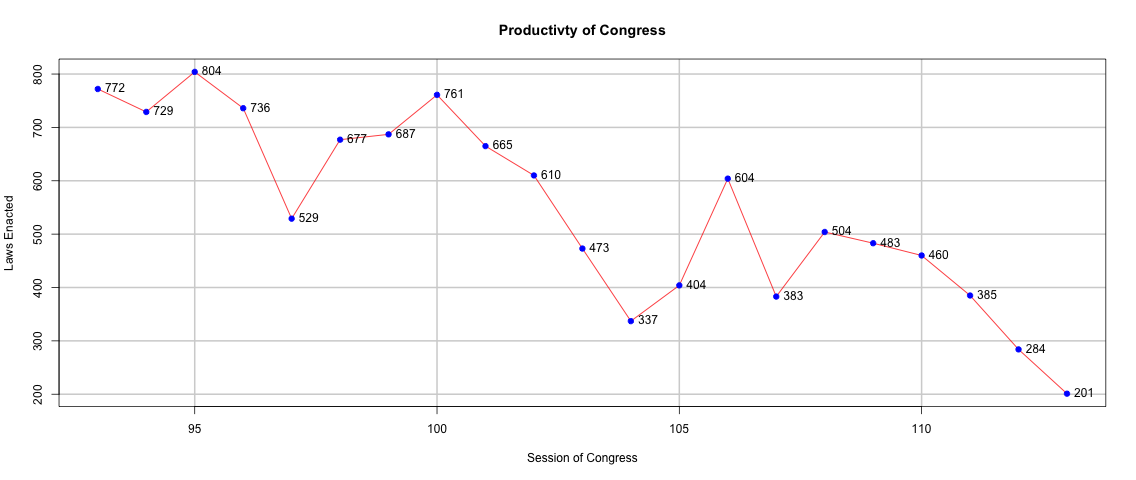
\includegraphics[width=\textwidth]{../prodCon.png}
		\caption*{Figure 1}
	\end{subfigure}
\end{figure}
On the other hand it could be that what would have been a temporary dip in productivity as been urged on by politically extreme members of the House of Representatives on both sides. It is clear from Figure 2 that there are strong trends towards the more extreme representative having more influence on both sides of the aisle. 
\begin{figure}[H]
	\centering
	\begin{subfigure}[H]{.4\textwidth}
		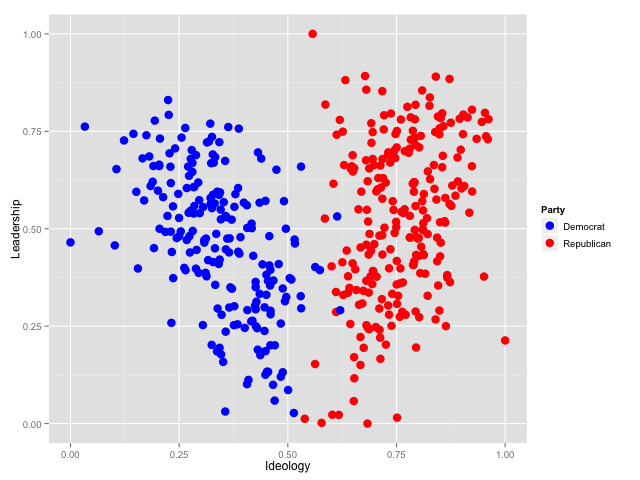
\includegraphics[width=\textwidth]{../charts/113chart.png}
		\caption*{Figure 2}
	\end{subfigure}
\end{figure}
Were we able to show that this circumstance is unique to the most recent sessions of Congress it would be reasonable to conclude that having ideologically extreme politicians in positions of great influence has contributed to the virtual halt in legislation. It is our hypothesis that this is the case. 
\section*{Literature Review}
To perform this analysis we will rely heavily on the academic works of a few authors. Each of these books are cited and can be found in the reference section at the end paper. Of particular interest are the books \textit{Applied Spatial Data Analysis with R}, which gives a thorough treatment of Generalized Additive models, \textit{Pattern Recognition and Machine Learning}, which was incredibly helpful with Principal Component Analysis, \textit{Elements of Statistical Learning}, a great resource on Generalized Additive models as well as Google's PageRank algorithm, and the fourth chapter of \textit{Google's PageRank and Beyond: The Science of Search Engine Rankings}, a very insightful look at Google's PageRank algorithm. I also used \textit{Data Analysis and Statistics for Geography, Environmental Science, and Engineering} as a general reference and great guide with the Linear models.
\section*{Acquisition and Processing of the Data}
\subsection*{Source of the Data}
The Congressional cosponsorship data that we will be using is from Joshua Tauberer and his website {\color{blue}\href{http://govtrack.us}{GovTrack.us}}. In 2004, Tauberer founded GovTrack.us and used the cosponsorship data to establish leadership and ideological scores for each Senator and Representative of Congress from the 93rd Congress forward. The method of generating these metrics will be discussed at a further point in the paper. Tauberer has made the data on his website freely available with an open API and bulk downloading options. \\
\\
This data was downloaded accessed using both bulk download and accessing the API. To download all of the data I used a bash script. Accessing the API was done through use of REST http requests. The responses were in JSON so the data was then parsed so that it could be read into R. The source code for this project can be located at {\color{blue}\href{http://www.github.com/howardgershon}{my GitHub site}} in the {\tt house\_analytics} repository.  
\subsection*{Preprocessing of the Data}
The cosponsorship data was used by Tauberer and GovTrack.us to extract information about how ideologically extreme each of the Representatives in the House are. To do this they employed Principle Component Analysis. Principle Component Analysis is the process of subtracting the mean out of each row of a dataset and examining the eigensystem of the covariance matrix of that dataset. Mathematically speaking, we create this covariance matrix thusly $$\mathbf{C} = \frac{1}{N}\sum_{n=1}^N(\mathbf{x}_n - \bar{\mathbf{x}})(\mathbf{x}_n - \bar{\mathbf{x}})^T$$ where $\mathbf{x}_n$ is each data point (in this case the information about the representative's cosponsorship behavior) and $\bar{\mathbf{x}}$ is the sample mean. The largest eigenvector of $\mathbf{C}$, $\lambda_1^\mathbf{C}$, is known as the first principal component. \cite{Bish01}\cite{Hast02} I have written a short function for it shown below. 
\begin{spacing}{1}
\newpage
\lstinputlisting[label=,caption={\asciifamily pca.r}]{../code/pca.r}
\end{spacing}
Performing this algorithm on the covariance of the mean adjusted cosponsorship matrix gave each of the representatives an ideology score. \\

The cosponsorship matrix was also used to generate a leadership score for each of the representatives. To produce this Tauberer used Google's PageRank algorithm. This is defined as $$\mathbf{\pi}^T = \mathbf{\pi}^T(\alpha\mathbf{S}+(1-\alpha)\mathbf{E})$$ where $\mathbf{S}$ is a stochastic matrix describing the cosponsorship graph, $\mathbf{E} = 1/n\mathbf{e}\mathbf{e}^T$ is another stochastic matrix and $\alpha$ is the probability of moving from one node to another. The vector $\mathbf{\pi}^T$ is called the invariant probability vector.\cite{Lawl01} Solving this numerically requires that this equation be treated as an update and performed repeatedly as $$\mathbf{\pi}^T_{k+1} = \mathbf{\pi}^T_k(\alpha\mathbf{S}+(1-\alpha)\mathbf{E})$$ until $\mathbf{\pi}^T_{k+1} = \mathbf{\pi}^T_k$ within some tolerance. In this case the cosponsorship matrix was already $\mathbf{P}(\alpha\mathbf{S}+(1-\alpha)\mathbf{E})$ which makes the entire algorithm easier. It is just \mathbf{\pi}^T_{k+1} = \mathbf{\pi}^T_k\mathbf{P}$ \cite{Lang01} The code for this algorithm is below.
\begin{spacing}{1}
\\
\lstinputlisting[label=,caption={\asciifamily pagerank.r}]{../code/pagerank.r}
\end{spacing}
The invariant probability vector is a vector of the leadership scores of each representative. 
\begin{figure}[p]
    \vspace*{-2cm} %\hspace*{-2cm}
    \makebox[1\linewidth]{
  		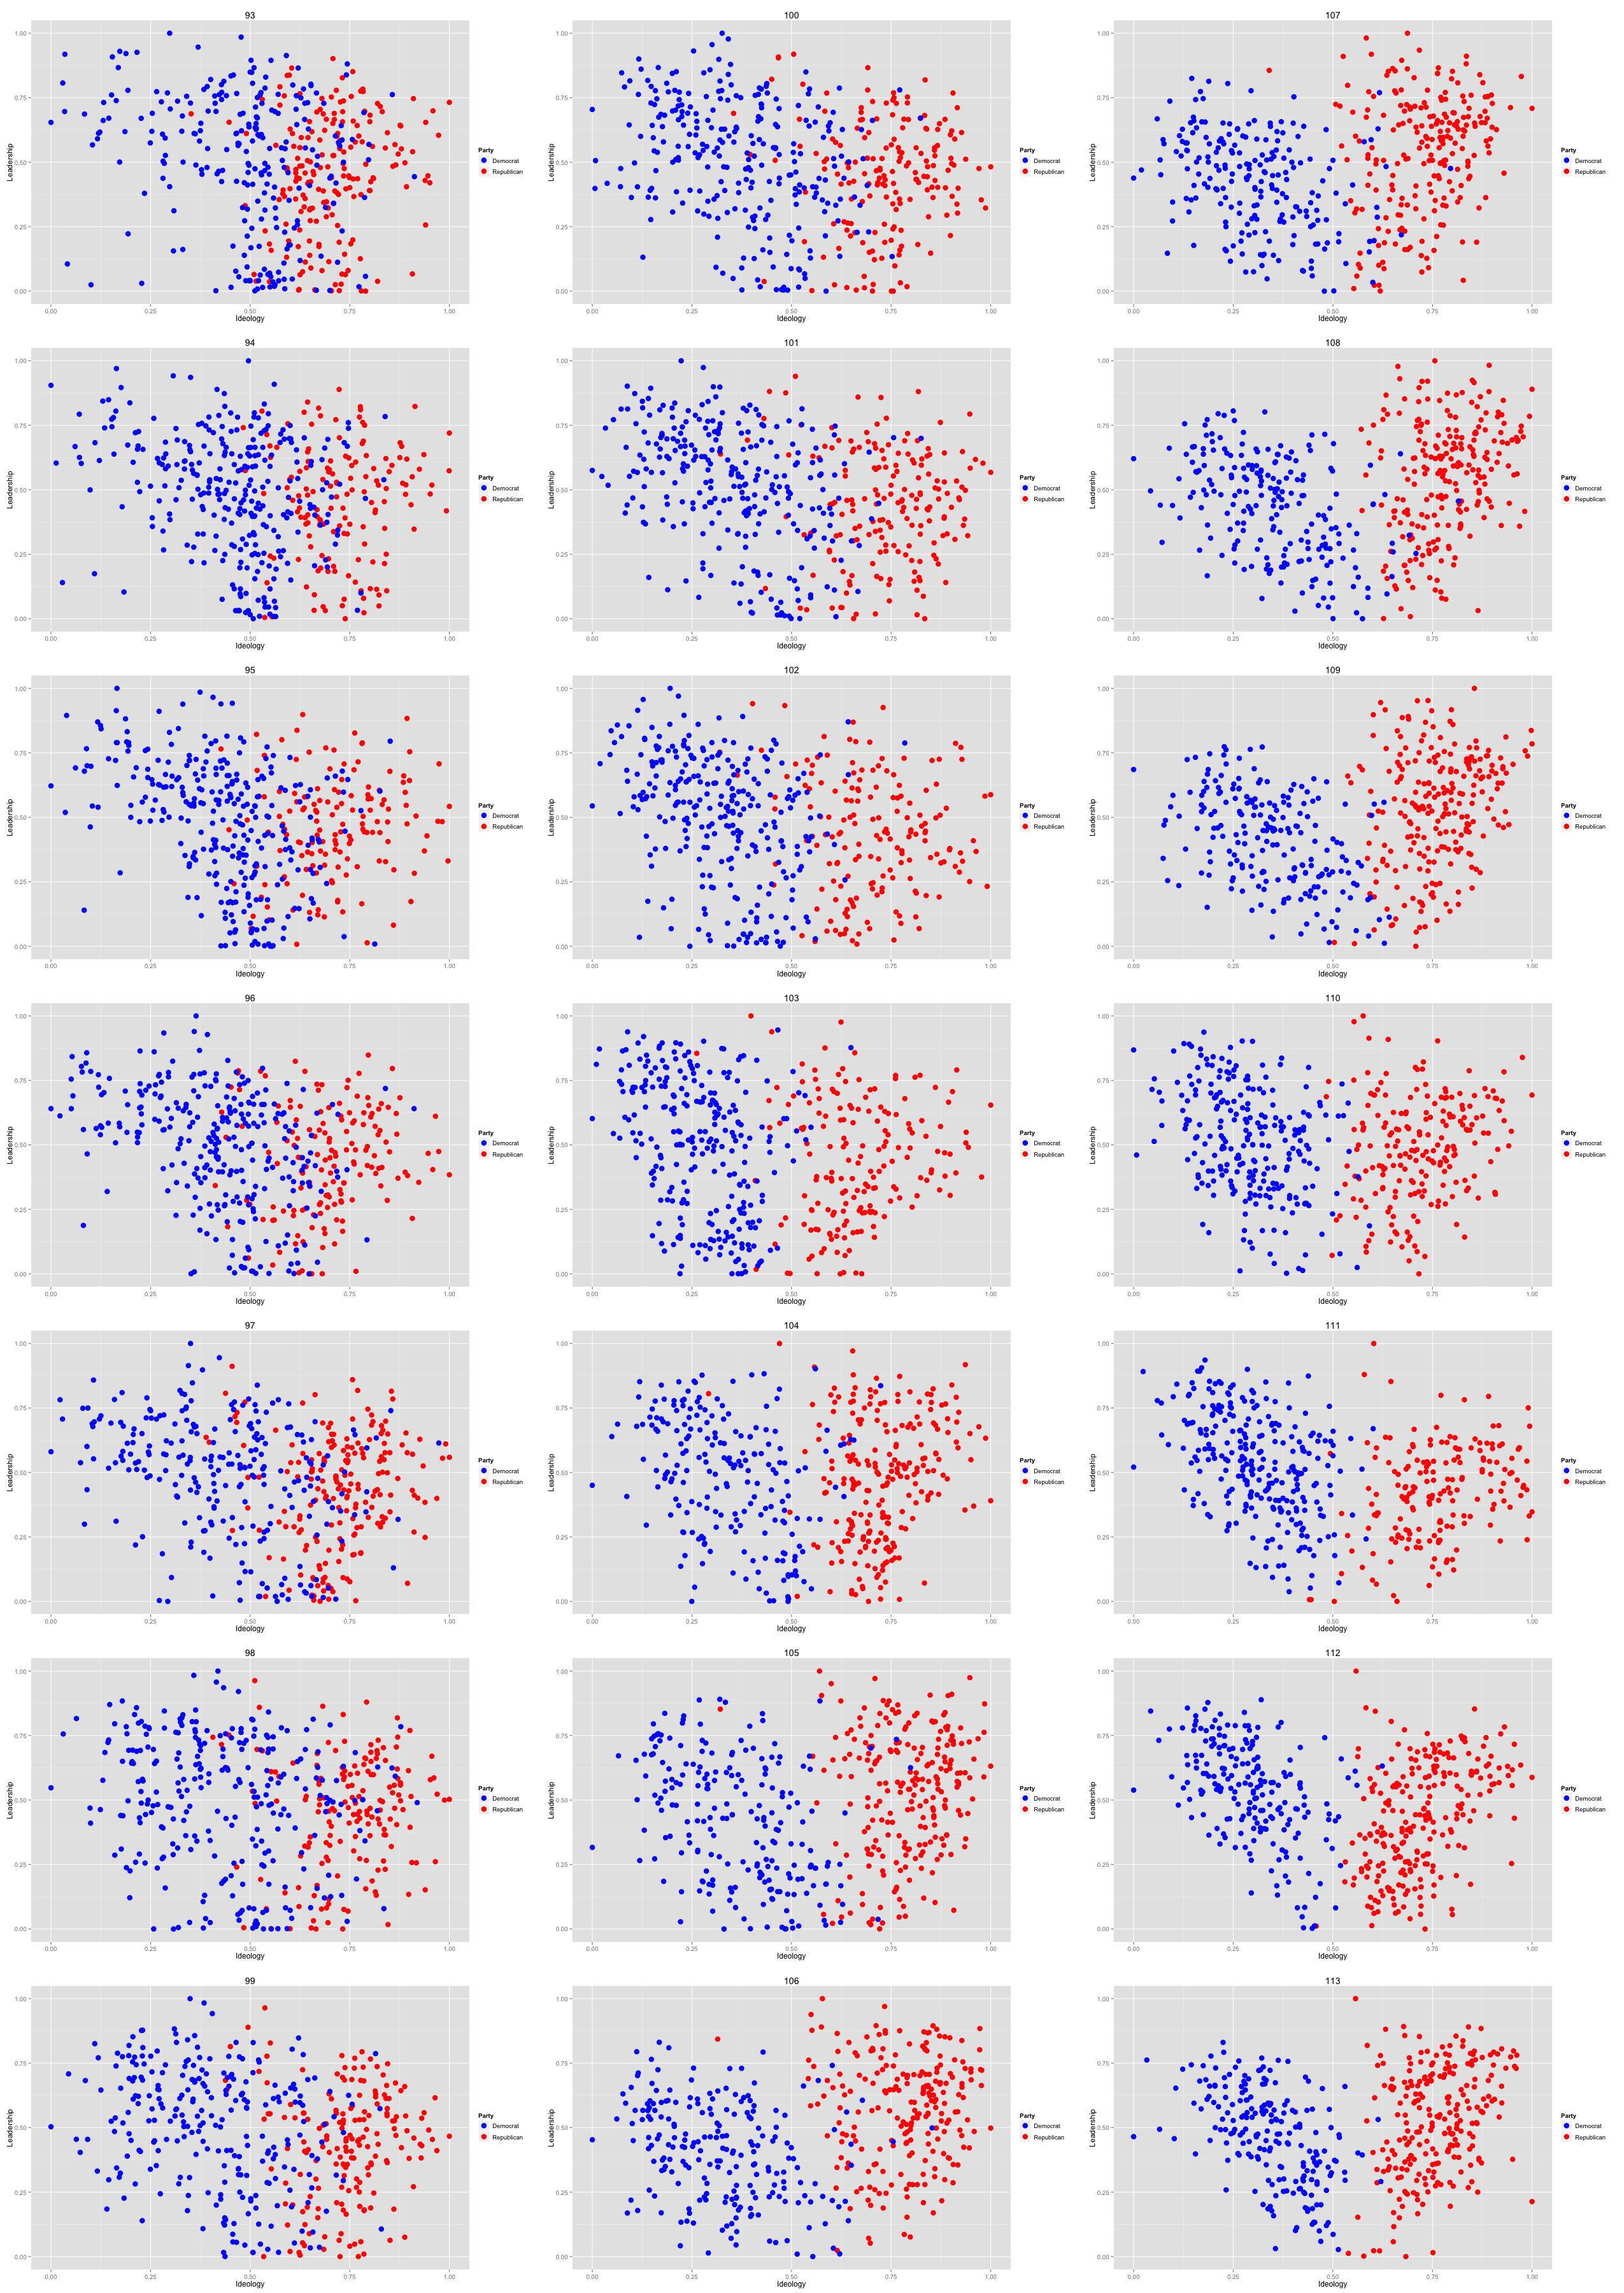
\includegraphics[width=1.2\linewidth]{../full.png}  	
    }
    \caption*{Figure 3 \\ Starts at top left and goes down each column}
\end{figure}
\section*{Statistical Methods}
My initial analysis of this data was to first produce plots of each of the points for each representative in each session of Congress. These point clouds can be seen on the next page. Looking at each of these point clouds you can certainly see that there is an emerging trend towards polarization in each of the parties. This lead me to use a linear model to regress the data set for each of these sessions of Congress to better how ideology scores are interacting with the leadership scores. 
\subsection*{Linear Model}
To look at the linear regression I used this model $$\mathbf{Y}_{\text{lead}} = \beta_0 + \beta_1\mathbf{X}_{\text{ideo}}$$ where $\beta_0$ is the intercept and $\beta_1$ is the slope of the regression.\cite{Acev01} Using this I then plotted the slopes in Figure 4. This shows the changing of the slopes with a higher slope meaning that the more extreme members of the House are the more powerful and a lower or negative slope meaning that more of the centrist members of the House are wielding more power. Figure 4 seems to communicate that the though the Republican party begins with a lower, more centrist-driven population they soon meet the Democratic party and surpass them in the 106th Congress ('99-'01). However the Republicans merely come up to meet the Democrats, surpass them only slightly, and oscillate between the Democrat's level and a lower level. Though this supports the claim that the Republicans are the party that is becoming more uncooperative, this also shows that the Democrats have always been there. \\
\begin{figure}[H]
	\centering
	\begin{subfigure}[H]{.4\textwidth}
		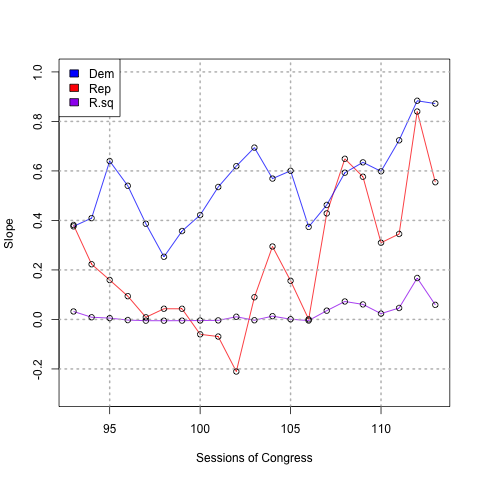
\includegraphics[width=\textwidth]{../lin.png}
		\caption*{Figure 4}
	\end{subfigure}
\end{figure}
You will notice the purple line. This is the $R^2$ values of each linear model for each year. These values are quite low. This can be explained by how dispersed the point clouds. This can be seen in Figure 3. As the low $R^2$ values are quite low, I decided to move to  a different model that more completely takes into account factors that could be introducing some dependent. 
\subsection*{Generalized Additive Model}
The dependencies that I was worried about were in the location of each of the representatives. I made the assumption that representatives that were in close proximity to each other would have leadership and ideological scores that were highly correlated. To lessen the effect of this on my model I added a bivariate spline $s(lat, lon)$.\cite{Biva01}\cite{Hast01} I also wanted to see if there were dependencies introduce by the sessions, or in other words if each session was closely correlated to the sessions that immediately surrounded it. To explore this I introduced a univariate spline $s(session)$. Combining these terms with my linear model we have $$\mathbf{Y}_{\text{lead}} = \beta_0 + \beta_1\mathbf{X}_{\text{ideo}}+s(lat, lon)+s(session).$$ The results of this model are seen in Figures 5 and 6. 
\begin{figure}[H]
	\centering
	\begin{subfigure}[H]{.4\textwidth}
		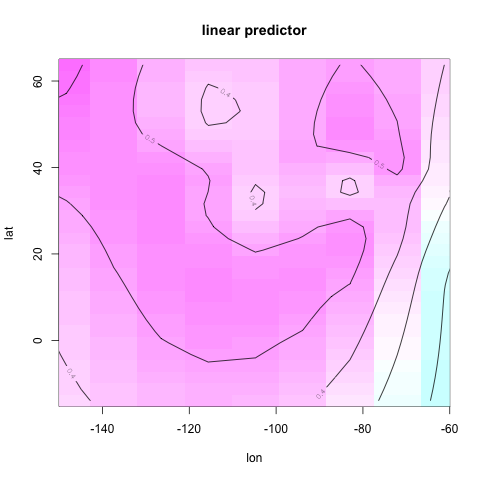
\includegraphics[width=\textwidth]{../gam.png}
		\caption*{Figure 5}
	\end{subfigure}
	\begin{subfigure}[H]{.4\textwidth}
		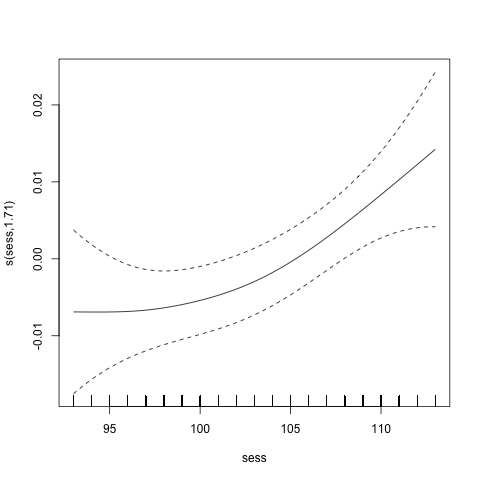
\includegraphics[width=\textwidth]{../gam2.png}
		\caption*{Figure 6}
	\end{subfigure}
\end{figure}
As you can see, in Figure 5, there seem to be high levels of leadership along the West Coast and in New England. These are more highly populated areas and therefore there are more representatives for these communities. We see that there are very low leadership scores in the Midwest. These states have lower populations and therefore fewer representatives. This seems to suggest that representatives that are closer in proximity to other representatives are more powerful. One explanation for this is that there is probably more opportunity for these representatives to work together. This points to the increasing urbanization of our society being a strong factor in the polarizing of our politicians. This position is supported by the strong and consistent polarization of the Democratic party, as the Democratic party is represented more in urban areas. Figure 6 confirms the upward trend towards polarization over time that we saw in the linear model. 
\subsection*{Categorical Analysis}
The final type of analysis that I am looking at is a categorical model that I set up. Looking at each the point cloud of just one party we could separate it into four quadrants based on the historical mean of the ideological score as the $y$-axis and the historical mean of the leadership score as the $x$-axis. This is illustrated in Figure 7 with the quadrants labeled 1 through 4. These labels are in reverse order for the Democrats because of the symmetric nature of the graph. Using this arrangement I categorized all of the data points and placed them on maps. In order to simplify this analysis I have restricted my maps to the continental Unites States. I want to focus on just a few of the sessions of Congress that I think show a down turn in productivity; the 95th ('77-'79), the 100th ('87-'89), and the 108th Congresses ('03-'05). You can see these maps in Figures 8, 9, and 10 respectively. 
\begin{figure}[H]
	\centering
	\begin{subfigure}[H]{.4\textwidth}
		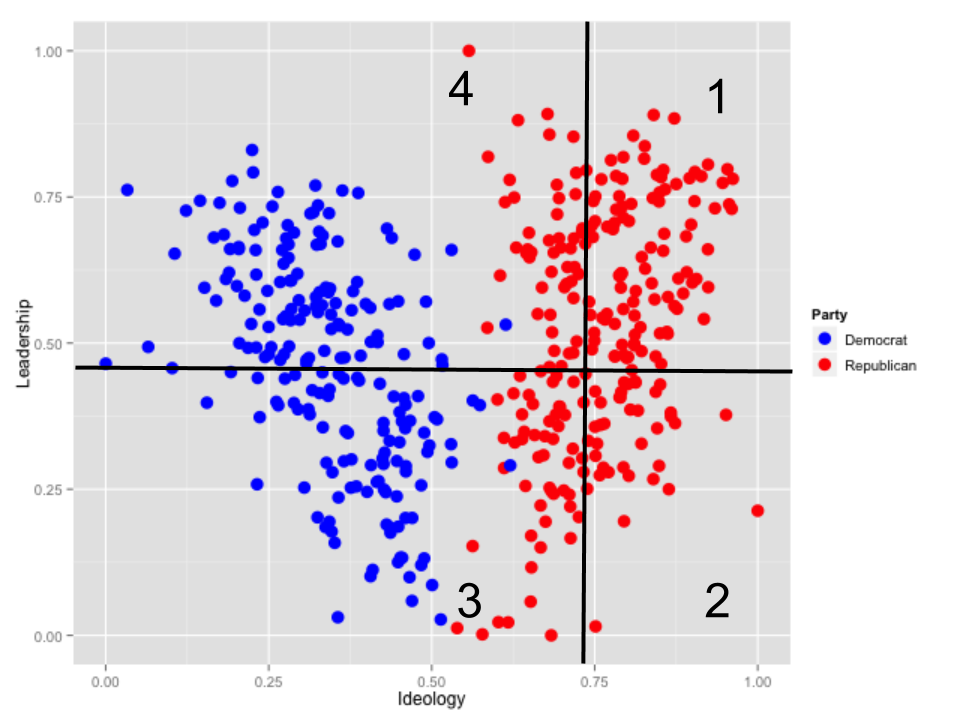
\includegraphics[width=\textwidth]{../quadrant.png}
		\caption*{Figure 7}
	\end{subfigure}
\end{figure}
These figures show that there were much fewer representatives that were in quadrant 1, the most polarized quadrant, in the 95th and 100th sessions. However these were sessions that started downward trends in productivity of the House (see Figure 1). This was also a time when the Republicans in the house were trending downward in their polarity and centrists in the party were becoming more powerful. The 108th congress, however, contrasts this. Each party is at the height of their polarization and there are more representative in quadrant one than ever.
\begin{figure}[H]
	\centering
	\begin{subfigure}[H]{.4\textwidth}
		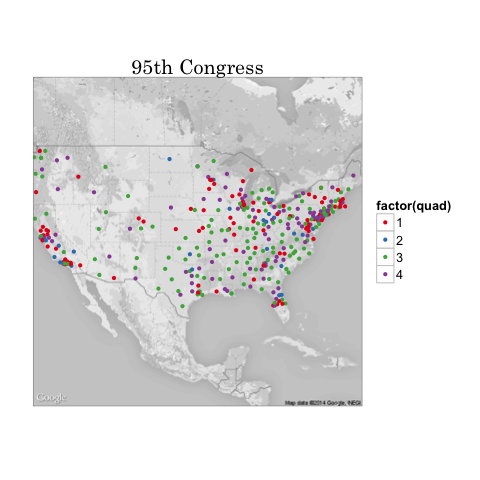
\includegraphics[width=\textwidth]{../map95.png}
		\caption*{Figure 8}
	\end{subfigure}
	\begin{subfigure}[H]{.4\textwidth}
		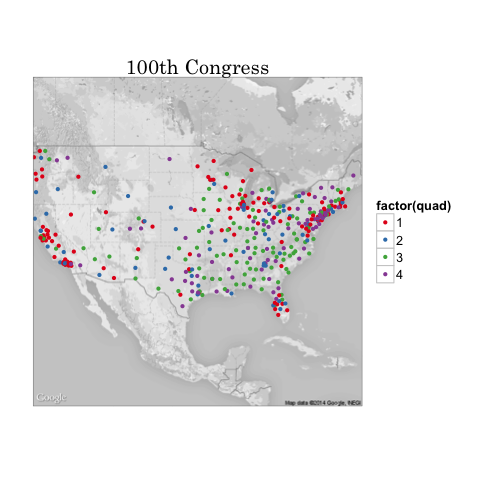
\includegraphics[width=\textwidth]{../map100.png}
		\caption*{Figure 9}
	\end{subfigure}
	\begin{subfigure}[H]{.5\textwidth}
		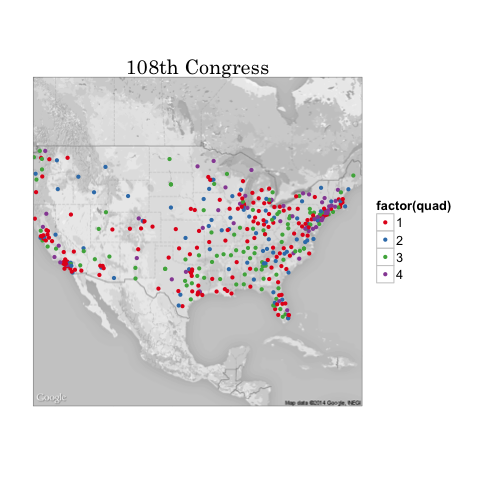
\includegraphics[width=\textwidth]{../map108.png}
		\caption*{Figure 10}
	\end{subfigure}
\end{figure}
In looking at the historical means of each of the parties I also looked at how those means have changed over time (Figures 11 and 12). I have also used a variant of a rose plot to look at the change in mean over time (Figures 13 and 14). These changes in means were almost completely opposite of each other between the two parties. Notice that reassignment of the number of representatives, which happens with each new census does not really have an effect on these changes. 
\begin{figure}[H]
	\centering
	\begin{subfigure}[H]{.8\textwidth}
		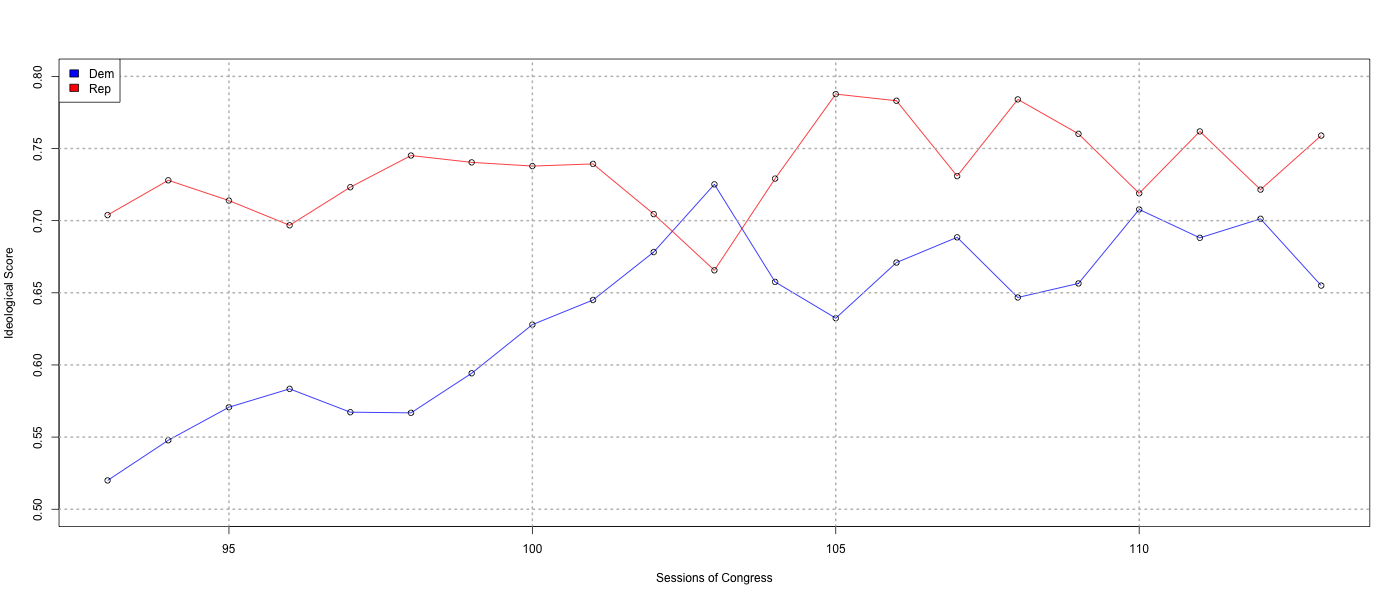
\includegraphics[width=\textwidth]{../IdeoMean.png}
		\caption*{Figure 11}
	\end{subfigure}
\end{figure}
\begin{figure}[H]
	\centering
	\begin{subfigure}[H]{.8\textwidth}
		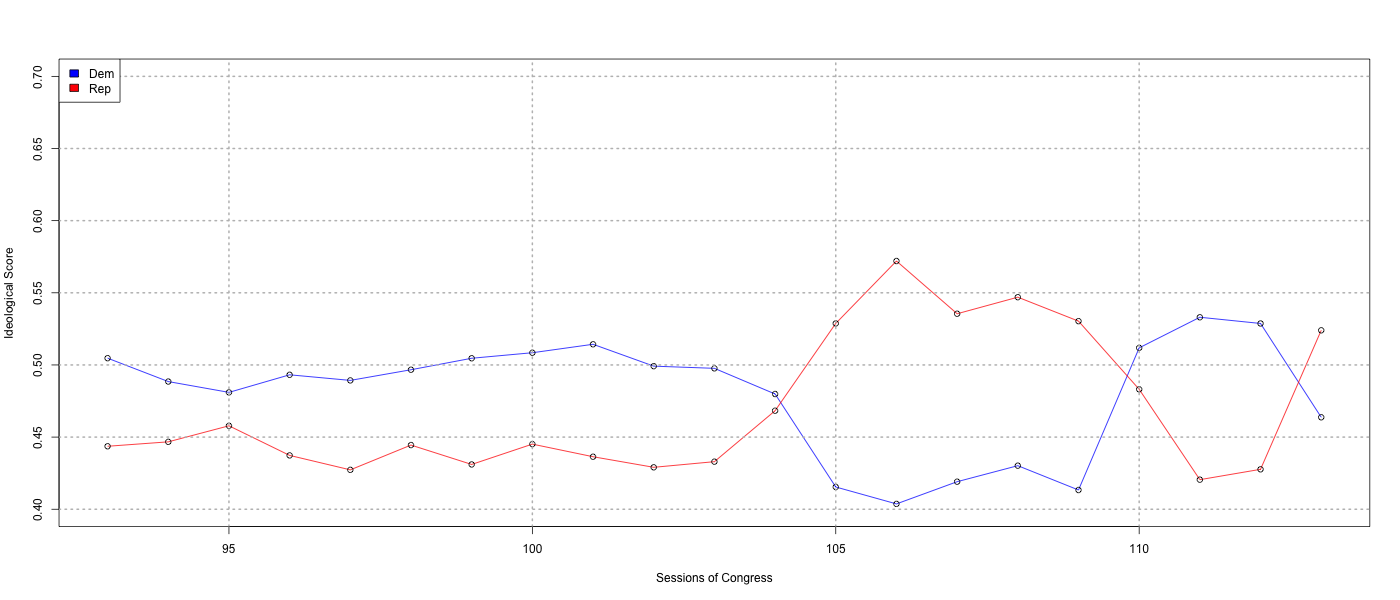
\includegraphics[width=\textwidth]{../LeadMean.png}
		\caption*{Figure 12}
	\end{subfigure}
\end{figure}
\begin{figure}[H]
	\centering
	\begin{subfigure}[H]{.45\textwidth}
		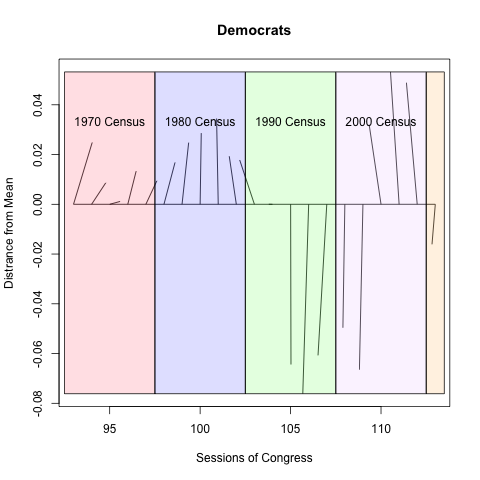
\includegraphics[width=\textwidth]{../meanDistDem.png}
		\caption*{Figure 13}
	\end{subfigure}
	\begin{subfigure}[H]{.45\textwidth}
		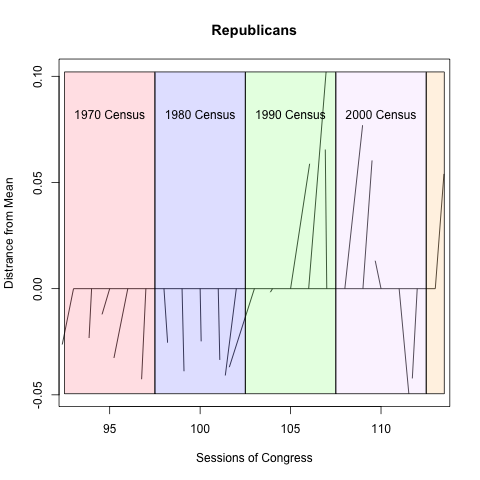
\includegraphics[width=\textwidth]{../meanDistRep.png}
		\caption*{Figure 14}
	\end{subfigure}
\end{figure}
\section*{Conclusion}
In conclusion, it seems that the idea that the lack of productivity of Congress because of either President Obama's administration or the rise of Tea Party is not completely accurate. From Figure 1 we can see that this unfortunate trend is much older than either of those factors. Without the uptick of legislation immediately following the attacks on the World Trade Center towers in 2001 the downward trend would have continued from 1999 until present day. Additionally this is not the first time we will have seen this type of down turn. From the data this is something that happens and gets better and then happens again and is worse that before. It is a general trend towards a completely stale mated Congress. The data that we are look at here is showing that there is a geographic component to this problem. In other words, as people move into urban areas their politicians become more polarized and less like to work with politicians across the aisle. This could also be due to people self-segregating. Moving not only into urban areas but also into areas that better represent their political views. Either way the data does not suggest a bright future. 
% Bibliography
\newpage
\begin{thebibliography}{7\kern\bibindent} 
\makeatletter
\let\old@biblabel\@biblabel
\def\@biblabel#1{\old@biblabel{#1}\kern\bibindent}
\let\old@bibitem\bibitem
\def\bibitem#1{\old@bibitem{#1}\leavevmode\kern-\bibindent}
\makeatother

	\bibitem{Acev01} Acevedo, Miguel F. Data Analysis and Statistics for Geography, Environmental Science, and Engineering. Boca Raton: CRC, 2013. Print.
	\bibitem{Bish01} Bishop, Christopher M. Pattern Recognition and Machine Learning. New York: Springer, 2006. Print.
	\bibitem{Biva01} Bivand, Roger, Edzer J. Pebesma, and Virgilio G�mez-Rubio. Applied Spatial Data Analysis with R. New York: Springer, 2008. Print.
	\bibitem{Hast01} Hastie, Trevor, and Robert Tibshirani. "Generalized Additive Models." Statistical Science 1.3 (1986): 297-310. Web.
	\bibitem{Hast02} Hastie, Trevor, Robert Tibshirani, and J. H. Friedman. The Elements of Statistical Learning: Data Mining, Inference, and Prediction. New York: Springer, 2009. Print.
	\bibitem{Lang01} Langville, Amy N., and C. D. Meyer. "Chapter 4: The Mathematics of Google's PageRank." Google's PageRank and Beyond: The Science of Search Engine Rankings. Princeton, NJ: Princeton UP, 2006. 31-46. Print.
	\bibitem{Lawl01} Lawler, Gregory F. Introduction to Stochastic Processes. New York: Chapman & Hall, 2006. Print.
\end{thebibliography}


\end{document}
